\section{Fingers Assembly}

This section contains instructions for assembling all 5 fingers of the prosthetic hand. Before each assembly step, a table containing all required materials and tools will be provided for convenience.

\subsection{Assembling the Phalanges}

%The parts and the materials you will need to assemble the fingers are listed in table \ref{phalangespartsmaterials}. The phalanges for all fingers of the hand can be assembled by gluing the parts of the following table, following the illustrated instructions of the the figures below. 

\begin{table}[ht!]
	\centering
	%\begin{minipage}[b]{0.50\linewidth}\centering
		\scalebox{1}{
			\begin{tabular}{ | c | c |}
				\hline
				\multicolumn{2}{|c|}{\bf{Part List 6.1.1}} \\
				\hline
				{\bf{Part Name}} & {\bf{Qty}}\\ \hline
				index & 1  \\ \hline
				middle & 1  \\ \hline
				ring & 1  \\ \hline
				pinky & 1  \\ \hline
				thumb & 1 \\ \hline
				tubeMIP & 8  \\ \hline
				tubePIP & 10  \\ \hline
				tubeDIP & 10  \\ \hline
				%		M3Washer & 16 \\ \hline
				%		M3Nut & 4 \\ \hline
				%		pulley & 4 \\ \hline
				\multicolumn{2}{|c|}{\textbf{Materials}} \\
				\hline
				\multicolumn{2}{|c|}{Super Glue } \\				
				\hline
			\end{tabular}				
		}
	%\end{minipage}
	
	%\caption{Parts and materials needed to assemble the phalanges.}
	%\label{phalangespartsmaterials}
\end{table}

%\begin{table}[ht!]
%	\centering
%	%\begin{minipage}[b]{0.50\linewidth}\centering
%
%	%\end{minipage}
%\end{table}



\begin{figure}[h]
	\centering
	\begin{tikzpicture}
	\node [mybox] (box){%
		\begin{minipage}[b]{0.45\textwidth}%\centering
		\begin{tabular}{ l l}
		{\circled{1}} & {Insert the low friction tubes to}\\
		{} & {the tubePIP/tubeMIP plates.} \\ \\
		{\circled{2}} & {Glue the edges of the tubes to}\\
		{} &  {the tube plates with super glue.}\\
		\end{tabular}
		\end{minipage}
		%\hspace{0.5cm}	
		\begin{minipage}[b]{0.4\textwidth}
		\begin{tabular}{ l }
		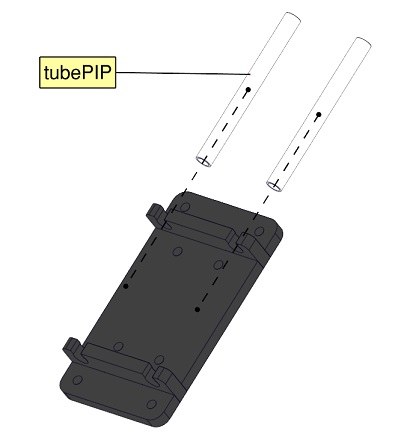
\includegraphics[width=6cm]{figures/Finger/Finger8.jpg}
		\end{tabular}
		\end{minipage}
	};
	%\node[anchor=south] at (-5,3.7) {\textbf{PIP and MIP Phalanges}}; % or (current bounding box.north) {Some Text};
	\node[mytitle, right=10pt] at (box.north west) {Board 6.1.1: Assembling PIP/MIP Phalanges};
	\end{tikzpicture}%
\end{figure}




\begin{figure}[!htbp]
	\centering
	\begin{tikzpicture}
	\node [mybox] (box){%
		\begin{minipage}[b]{0.45\linewidth}
		\begin{tabular}{l l}
		{\circled{1}} & {Insert the low friction tubes to the}\\
		{} & {tubeDIP plate.} \\ \\
		{\circled{2}} & {Glue the edges of the tubes to the}\\
		{} &  {tubeDIP plate with super glue.}\\
		\end{tabular}
		\end{minipage}
		%\hspace{0.5cm}	
		\begin{minipage}[b]{0.45\linewidth}
		\begin{tabular}{ l }
		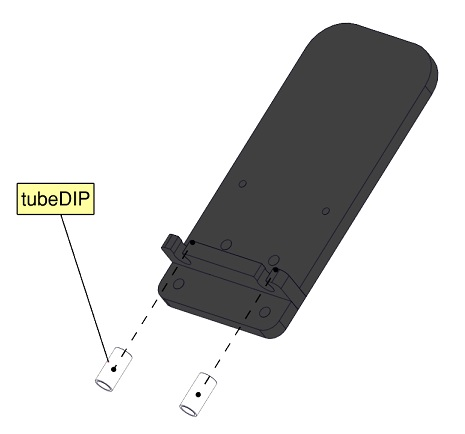
\includegraphics[width=6cm]{figures/Finger/Finger10.jpg}
		\end{tabular}
		\end{minipage}
	};
	\node[mytitle, right=10pt] at (box.north west) {Board 6.1.2: Assembling DIP Phalange};
	\end{tikzpicture}%
\end{figure}

\begin{figure}[h]
	\centering
	\begin{tikzpicture}
	\node [mybox] (box){%
		\begin{minipage}[b]{.3\textwidth}
		\begin{tabular}{ c }
		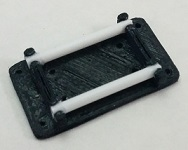
\includegraphics[width = 3cm]{figures/Finger/Finger11.jpg}
		\end{tabular}
		\end{minipage}	
		\begin{minipage}[b]{0.3\textwidth}
		\begin{tabular}{ c }
		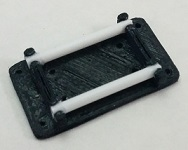
\includegraphics[width = 3cm]{figures/Finger/Finger11.jpg}
		\end{tabular}
		\end{minipage}
		\begin{minipage}[b]{0.3\textwidth}
		\begin{tabular}{ c }
		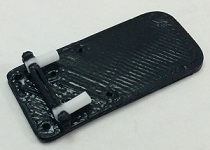
\includegraphics[width = 3.4cm]{figures/Finger/Finger12.jpg}
		\end{tabular}
		\end{minipage}
	};
	\node[anchor=south] at (5.5,-1.2) {\textbf{DIP}};
	\node[anchor=south] at (0.5,-1.2) {\textbf{MIP}};
	\node[anchor=south] at (-4,-1.2) {\textbf{PIP}};	
	\node[mytitle, right=10pt] at (box.north west) {Board 6.1.3: Completed Phalanges};
	\end{tikzpicture}%
\end{figure}

\newpage


\subsection{Attaching the Phalanges on the Flexure Joints }

The flexure joints of each finger are implemented with silicone sheets, attached to each pair of neighboring phalanges via simple stitching with nylon fishing line and long needles as shown in the following assembly steps. 


\begin{table}[ht!]
	\centering
		\centering
		\scalebox{1}{
			\begin{tabular}{ | c | c |}
				\hline
				\multicolumn{2}{|c|}{{\textbf{Part List 6.2.1}}} \\\hline								
				{\bf{Par Namet}} & {\bf{Qty}}\\ \hline
				index & 1  \\ \hline
				middle & 1  \\ \hline
				ring & 1  \\ \hline
				pinky & 1  \\ \hline
				thumb & 1 \\ \hline
				Joint DIP \& MIP & 4  \\ \hline
				Joint PIP & 5  \\ \hline
				\multicolumn{2}{|c|}{{\textbf{Tools}}} \\\hline				
				\multicolumn{2}{|c|}{{{Long Needles}}} \\\hline
				\multicolumn{2}{|c|}{{Nylon Fishing Line}} \\\hline
				\multicolumn{2}{|c|}{{{Cutter}}} \\\hline
				\multicolumn{2}{|c|}{{{Long-Nose Pliers with Side-Cutting}}} \\\hline
				\multicolumn{2}{|c|}{{{Precision Ruler}}} \\\hline
				\multicolumn{2}{|c|}{{{Scissors}}} \\\hline
			\end{tabular}
		}
	%\caption{Parts and tools needed to attach the phalanges to the flexure joints.}
	%\label{attachingparts}		
\end{table}

%	\begin{minipage}[b]{0.45\linewidth}
%		\centering
%		\scalebox{1}{
%			\begin{tabular}{ | c |}
%				\hline
%				\multicolumn{1}{|c|}{{\bf{Tools}}} \\
%				\hline
%				Long Needles \\ \hline
%				Nylon Fishing Line \\ \hline
%				Cutter \\ \hline
%				Long-Nose Pliers with Side-Cutting \\ \hline
%				Precision Ruler \\ \hline
%				Scissors \\ \hline
%			\end{tabular}
%		}
%	\end{minipage}	

Board 6.2.1 displayes an overview of the stitching patterns. The red lines denote stitching that passes from both sides of the rigid part and the flexure joint, while the blue lines depict a fishing line that passes only from the lower side of the flexure joint. 


\begin{figure}[h]
	\centering
	\begin{tikzpicture}
	\node [mybox] (box){%
		\begin{minipage}[b]{0.45\textwidth}
		\centering
		\begin{tabular}{ l }
		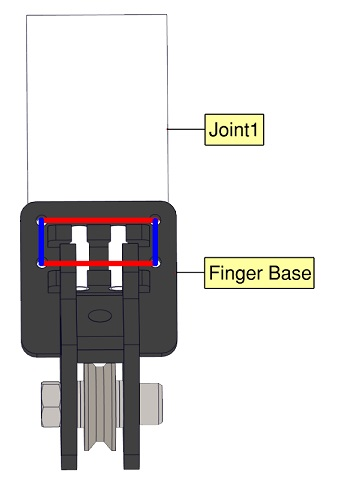
\includegraphics[width=4.5cm]{figures/Finger/Finger13.jpg}
		\end{tabular}
		\end{minipage}
		\begin{minipage}[b]{0.45\textwidth}
		\centering
		\begin{tabular}{ r }
		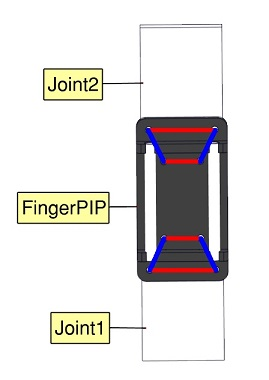
\includegraphics[width=4.5cm]{figures/Finger/Finger14.jpg}
		\end{tabular}
		\end{minipage}
	};	
	\node[mytitle, right=10pt] at (box.north west) {Board 6.2.1: Phalange/Joint Attachment Overview};
	\end{tikzpicture}%
\end{figure}

\newpage

The stitching steps are illustrated in the following figures.


\begin{center}
	\begin{tikzpicture}
	\node [mybox] (box){%
		\begin{minipage}[b]{0.45\linewidth}
		\begin{tabular}{ l }
		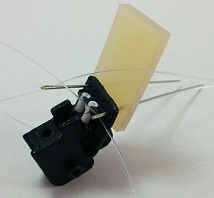
\includegraphics[width=6cm]{figures/Finger/Finger15.jpg} 
		\end{tabular}
		\end{minipage}
		\begin{minipage}[b]{0.45\linewidth}
		\begin{tabular}{ l l}
		{\circled{1}} &  {Cut 450mm of fishing line.}\\ \\
		{\circled{2}} & {Pass the fishing line through}\\
		{} &  {the eyes of the needles.}\\ \\
		{\circled{3}} & {Insert the needles into the upper,}\\
		{} & { and outer slots of PIP.}\\
		\end{tabular}
		\end{minipage}
	};
	\node[mytitle, right=10pt] at (box.north west) {Board 6.2.2: Stitching Step I};
	\end{tikzpicture}%
\end{center}


\begin{center}
	\begin{tikzpicture}
	\node [mybox] (box){%
		\begin{minipage}[b]{0.45\linewidth}
		\begin{tabular}{ l l }
		{\circled{1}} & {Pass each needle through the eye}\\
		{} &  {of the other.}\\ \\
		{\circled{2}} & {Repeat step \circled{1} twice.}\\ \\
		{\circled{!}} & {The needles are now in the lower}\\
		{} & {side of MIP.}\\ \\
		{\circled{3}} & {Insert the needles into the inner slots}\\ 
		{} &  {of MIP.} \\
		\end{tabular}
		\end{minipage}
		\begin{minipage}[b]{0.45\linewidth}
		\begin{tabular}{ l }
		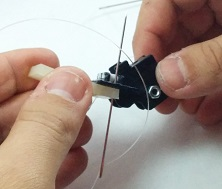
\includegraphics[width=6cm]{figures/Finger/Finger16.jpg}
		\end{tabular}
		\end{minipage}
	};
	\node[mytitle, right=10pt] at (box.north west) {Board 6.2.3: Stitching Step II};
	\end{tikzpicture}%
\end{center}


\begin{center}
	\begin{tikzpicture}
	\node [mybox] (box){%
		\begin{minipage}[b]{0.45\linewidth}
		\begin{tabular}{ l }
		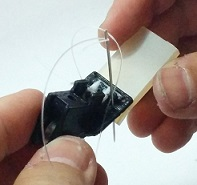
\includegraphics[width=6cm]{figures/Finger/Finger17.jpg} 
		\end{tabular}
		\end{minipage}
		\begin{minipage}[b]{0.45\linewidth}
		\begin{tabular}{ l l }
		{\circled{1}} & {Pass each needle from the eye of the}\\
		{} &  {other.} \\ \\
		{\circled{2}} & {Repeat step \circled{1} 3 times.}\\ \\
		{\circled{!}} & {The needles are now in the lower side}\\
		{} & {of MIP.}\\
		\end{tabular}
		\end{minipage}
	};
	\node[mytitle, right=10pt] at (box.north west) {6.2.4: Stitching Step III};
	\end{tikzpicture}%
\end{center}


\begin{center}
	\begin{tikzpicture}
	\node [mybox] (box){%
		\begin{minipage}[b]{0.55\linewidth}
		\begin{tabular}{ l l}
		{\circled{1}} & {Remove the needles from the}\\
		{} & {fishing line.} \\ \\
		{\circled{2}} & {Tie the ends of the fishing line}\\
		{} & {with multiple surgeon's knots.}\\
		\end{tabular}
		\end{minipage}
		\begin{minipage}[b]{0.35\linewidth}
		\begin{tabular}{ r }
		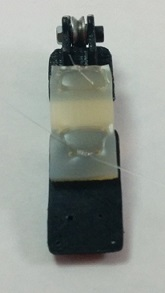
\includegraphics[width=3cm]{figures/Finger/Finger18.jpg}
		\end{tabular}
		\end{minipage}
	};
	\node[mytitle, right=10pt] at (box.north west) {Board 6.2.5: Stitching Step IV};
	\end{tikzpicture}%
\end{center}



\begin{center}
	\begin{tikzpicture}
	\node [mybox] (box){%
		\begin{minipage}[b]{0.45\linewidth}
		\begin{tabular}{ l l}
		{\circled{1}} & {Cut 450mm of fishing line.} \\ \\
		{\circled{2}} & {Pass the fishing line through}\\
		{} &  {the slots of two long needles.} \\ \\
		%		\circled{3} Center the fingerPIP part with the silicone part\\ and align it with the line from the previous step.\\
		{\circled{3}} &  {Insert the needles in the lower,}\\
		{} &  {outer holes of PIP.} \\
		\end{tabular}
		\end{minipage}
		\begin{minipage}[b]{0.45\linewidth}
		\begin{tabular}{ c }
		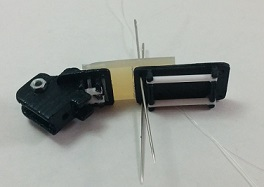
\includegraphics[width=6cm]{figures/Finger/Finger20.jpg} 
		\end{tabular}
		\end{minipage}
	};
	\node[mytitle, right=10pt] at (box.north west) {Board 6.2.6: Stitching Step V};
	\end{tikzpicture}%
\end{center}


\begin{center}
	\begin{tikzpicture}
	\node [mybox] (box){%
		\begin{minipage}[b]{0.45\linewidth}\centering
		\begin{tabular}{ l }
		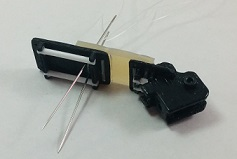
\includegraphics[width=6cm]{figures/Finger/Finger21.jpg}
		\end{tabular}
		\end{minipage}
		\hspace{0.5cm}	
		\begin{minipage}[b]{0.45\linewidth}
		\begin{tabular}{ l l}
		{\circled{1}} & {Pass each needle through the eye}\\
		{} & {of each other.} \\ \\
		{\circled{2}} & {Repeat step \circled{1} 3 times.} \\ \\
		{\circled{!}} &  {The needles are now in the lower}\\
		{} & {side of PIP.}\\
		\end{tabular}
		\end{minipage}
	};
	\node[mytitle, right=10pt] at (box.north west) {Board 6.2.7: Stitching Step VI};
	\end{tikzpicture}%
\end{center}



\begin{center}
	\begin{tikzpicture}
	\node [mybox] (box){%
		\begin{minipage}[b]{0.45\linewidth}\centering
		\begin{tabular}{ l l }
		{\circled{1}} & {Insert the needles into the inner,}\\
		{} & {lower slots of PIP.}\\ \\
		{\circled{2}} & {Pass each needle through the eye}\\
		{} & {of each other.}\\ \\
		{\circled{3}} & {Repeat step \circled{2} 3 times.}\\ \\
		{\circled{!}} & {The needles are now in the lower}\\
		{} &  {side of PIP.} \\ \\
		{\circled{4}} & {Remove the needles from the}\\
		{} &  {fishing line.}\\ \\
		{\circled{5}} & {Tie the ends of the fishing line}\\
		{} &  {with multiple surgeon's knots.}\\
		\end{tabular}
		\end{minipage}
		\hspace{0.5cm}	
		\begin{minipage}[b]{0.45\linewidth}
		\begin{tabular}{ c }
		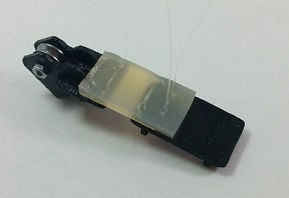
\includegraphics[width=6cm]{figures/Finger/Finger22.jpg}
		\end{tabular}
		\end{minipage}
	};
	\node[mytitle, right=10pt] at (box.north west) {Board 6.2.8: Stitching Step VII};
	\end{tikzpicture}%
\end{center}


\begin{center}
	\begin{tikzpicture}
	\node [mybox] (box){%
		\begin{minipage}[b]{0.45\linewidth}\centering
		\begin{tabular}{ l }
		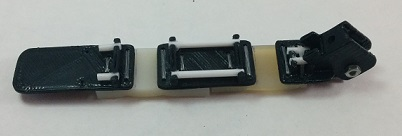
\includegraphics[width=7cm]{figures/Finger/Finger23.jpg}
		\end{tabular}
		\end{minipage}
		\hspace{0.5cm}	
		\begin{minipage}[b]{0.45\linewidth}
		\begin{tabular}{ l l}
		{\circled{1}} & {Repeat steps 6.2.5 - 6.2.7 for DIP.} \\ \\
		{\circled{!}} & {Congratulations, you built a finger!}
		\end{tabular}
		\end{minipage}
	};
	\node[mytitle, right=10pt] at (box.north west) {Board 6.2.9: Completed Finger};
	\end{tikzpicture}%
\end{center}

\newpage

\subsection{Tendon Routing System Assembly}


\begin{table}[h]
	\centering
	%\begin{minipage}[b]{0.50\linewidth}\centering
		\scalebox{0.97}{
			\begin{tabular}{ | c | c |}
				\hline
				\multicolumn{2}{|c|}{{\textbf{Part List 6.3.1}}} \\ \hline	
				{\bf{Part Name}} & {\bf{Qty}}\\ \hline
				index & 1  \\ \hline
				middle & 1  \\ \hline
				ring & 1  \\ \hline
				pinky & 1  \\ \hline
				thumb & 1 \\ \hline
				\multicolumn{2}{|c|}{{\bf{Tools \& Materials}}} \\ \hline
				\multicolumn{2}{|c|}{{Scissors}} \\ \hline
				\multicolumn{2}{|c|}{{Dyneema}} \\ \hline
				
				%		Precision Ruler \\ \hline
				
			\end{tabular}
		}	
\end{table}

\vspace{0.2cm}

\begin{center}
	\begin{tikzpicture}
	\node [mybox] (box){%
		\begin{minipage}[b]{0.45\linewidth}\centering
		\begin{tabular}{ c }
		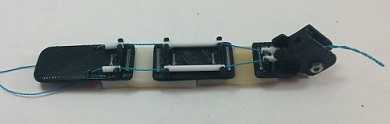
\includegraphics[width=7cm]{figures/Finger/Finger24.jpg}
		\end{tabular}
		\end{minipage}
		\hspace{0.5cm}	
		\begin{minipage}[b]{0.50\linewidth}
		\begin{tabular}{ l l}
		{\circled{1}} & {Cut 600mm of fishing line.} \\ \\
		{\circled{2}} & {Pass the Dyneema through the phalange}\\
		{} & {tubes starting from PIP.} \\
		\end{tabular}
		\end{minipage}
	};
	\node[mytitle, right=10pt] at (box.north west) {Board 6.3.1: Passing the Dynema from the Phalange Tubes};
	\end{tikzpicture}%
\end{center}

\vspace{0.2cm}

\begin{center}
	\begin{tikzpicture}
	\node [mybox] (box){%
		\begin{minipage}[b]{0.45\linewidth}\centering
		\begin{tabular}{ c }
		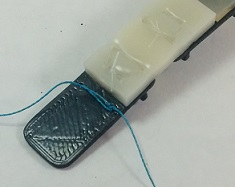
\includegraphics[width=7cm]{figures/Finger/Finger26.jpg}
		\end{tabular}
		\end{minipage}
		\hspace{0.5cm}	
		\begin{minipage}[b]{0.50\linewidth}
		\begin{tabular}{ l l }
		{\circled{1}} & {Tie the ends of Dyneema with}\\
		{} & {multiple \href{https://en.wikipedia.org/wiki/Surgeon%27s_knot}{surgeon's knots}.} \\
		\end{tabular}
		\end{minipage}
	};
	\node[mytitle, right=10pt] at (box.north west) {Board 6.3.2: Fixing the Dynema on the Fingers};
	\end{tikzpicture}%
\end{center}

\newpage

\subsection{Attaching the Soft Fingetips on the Fingers}

\begin{table}[ht!]
		\centering
		\scalebox{0.97}{
			\begin{tabular}{ | c | c |}
				\hline
				\multicolumn{2}{|c|}{{\textbf{Parts List 6.4.1}}} \\\hline	
				{\bf{Part Name}} & {\bf{Qty}}\\ \hline
				index & 1  \\ \hline
				middle & 1  \\ \hline
				ring & 1  \\ \hline
				pinky & 1  \\ \hline
				thumb & 1 \\ \hline
				\multicolumn{2}{|c|}{{\bf{Tools \& Materials}}} \\\hline
				\multicolumn{2}{|c|}{{Scissors}} \\ \hline
				\multicolumn{2}{|c|}{{Self-Adhesive Tape}} \\ \hline
				\multicolumn{2}{|c|}{{Deformable Spong-like Tape}} \\ \hline
				\multicolumn{2}{|c|}{{Anti-Slip Tape}} \\ \hline			
			\end{tabular}
		}	
\end{table}

\vspace{0.2cm}

\begin{center}
	\begin{tikzpicture}
	\node [mybox] (box){%
		\begin{minipage}[b]{0.45\linewidth}\centering
		\begin{tabular}{ c }
		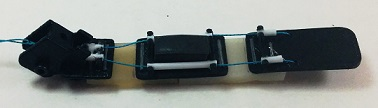
\includegraphics[width=7cm]{figures/Finger/Finger28.jpg}
		\end{tabular}
		\end{minipage}
		\hspace{0.5cm}	
		\begin{minipage}[b]{0.45\linewidth}
		\begin{tabular}{ l l }
		{\circled{1}} & {Cut two pieces of sponge-like tape}\\
		{} & {to the size of PIP.} \\ \\
		{\circled{2}} & {Attach the tape pieces on PIP.} \\
		\end{tabular}
		\end{minipage}
	};
	\node[mytitle, right=10pt] at (box.north west) {Board 6.4.1: PIP Inner Coating};
	\end{tikzpicture}%
\end{center}

\vspace{0.2cm}

\begin{center}
	\begin{tikzpicture}
	\node [mybox] (box){%
		\begin{minipage}[b]{0.45\linewidth}\centering
		\begin{tabular}{ l l}
		{\circled{1}} & {Cut 130mm of self-adhesive tape.} \\ \\
		{\circled{2}} & {Wrap the tape around PIP.} \\
		\end{tabular}
		\end{minipage}
		\hspace{0.5cm}	
		\begin{minipage}[b]{0.45\linewidth}
		\begin{tabular}{ c }
		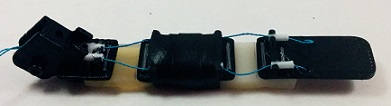
\includegraphics[width=6.5cm]{figures/Finger/Finger29.jpg}
		\end{tabular}
		\end{minipage}
	};
	\node[mytitle, right=10pt] at (box.north west) {Board 6.4.2: Fixing PIP Coating};
	\end{tikzpicture}%
\end{center}

\vspace{0.2cm}

\begin{center}
	\begin{tikzpicture}
	\node [mybox] (box){%
		\begin{minipage}[b]{0.45\linewidth}\centering
		\begin{tabular}{ c }
		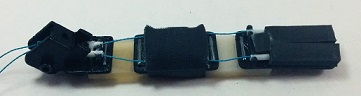
\includegraphics[width=7cm]{figures/Finger/Finger31.jpg}
		\end{tabular}
		\end{minipage}
		\hspace{0.5cm}	
		\begin{minipage}[b]{0.45\linewidth}
		\begin{tabular}{ l l}
		{\circled{1}} & {Cut two pieces of sponge-like tape}\\
		{} &  {to the size of DIP.} \\ \\
		{\circled{2}} & {Attach the pieces on DIP.} \\
		%		\circled{3} Cut a piece of 10mm sponge tape. \\
		%		\circled{4} Set the sponge tape onto the empty space \\ of the Finger DIP. \\
		%		\circled{5} Cut two pieces of 40mm sponge tape and \\ set them onto the other side.
		\end{tabular}
		\end{minipage}
	};
	\node[mytitle, right=10pt] at (box.north west) {Board 6.4.3: DIP Inner Coating};
	\end{tikzpicture}%
\end{center}

\vspace{0.2cm}

\begin{center}
	\begin{tikzpicture}
	\node [mybox] (box){%
		\begin{minipage}[b]{0.45\linewidth}\centering
		\begin{tabular}{ c }
		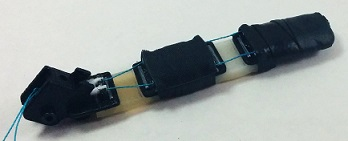
\includegraphics[width=7cm]{figures/Finger/Finger32.jpg}
		\end{tabular}
		\end{minipage}
		\hspace{0.5cm}	
		\begin{minipage}[b]{0.45\linewidth}
		\begin{tabular}{ l l }
		{\circled{1}} & {Cut 200mm of self-adhesive tape.} \\ \\
		{\circled{2}} & {Wrap the tape around the DIP.} \\
		\end{tabular}
		\end{minipage}
	};
	\node[mytitle, right=10pt] at (box.north west) {Board 6.4.4: Fixing DIP Coating};
	\end{tikzpicture}%
\end{center}

\newpage

\begin{center}
	\begin{tikzpicture}
	\node [mybox] (box){%
		\begin{minipage}[b]{0.4\linewidth}\centering
		\begin{tabular}{ l l }
		{\circled{1}} & {Cut a piece of anti-slip tape}\\
		{} & {to the size of PIP.} \\ \\
		{\circled{2}} & {Attach the tape on PIP.} \\ \\
		{\circled{3}} & {Cut a piece of anti-slip tape}\\
		{} & {to the size of DIP.} \\ \\
		{\circled{4}} & {Attach the tape on DIP.} \\ \\
		{\circled{!}} & {Cut the edges of the tape.} \\ \\
		\end{tabular}
		\end{minipage}
		\begin{minipage}[b]{0.53\linewidth}
		\begin{tabular}{ c }
		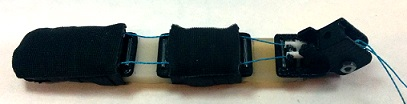
\includegraphics[width=8cm]{figures/Finger/Finger33.jpg}
		\end{tabular}
		\end{minipage}
	};
	\node[mytitle, right=10pt] at (box.north west) {Board 6.4.5: Anti-Slip Coating};
	\end{tikzpicture}%
\end{center}
